%\mychapter{6}{Results}

\section{Results}
In this section, we report our results on clean synthetic data
using diffusion maps with the $l_{1}$ distance. We compare our results with those obtained via PCA, a popular linear dimensionality technique. Figure \ref{fig:Output-on-SimFR} shows that diffusion maps  with $l_{1}$ distance appears to capture the animal's circular motion better than PCA when applied on firing rate data. Using previous time data, diffusion maps with $l_{1}$ data appears to outperform PCA, Figure \ref{fig:Output-on-SimPrevtime}.
We also see that using previous time data captures changes in spike timing
as the animal makes 4 laps around the circle.

\subsection{Simulation results on Firing Rate}
In this section, we show our fake-brain results using 
diffusion maps with the $l_1$-norm and PCA  on simulated firing rate.

\begin{figure}[h!]
\centering
\begin{subfigure}[b]{.45\linewidth}
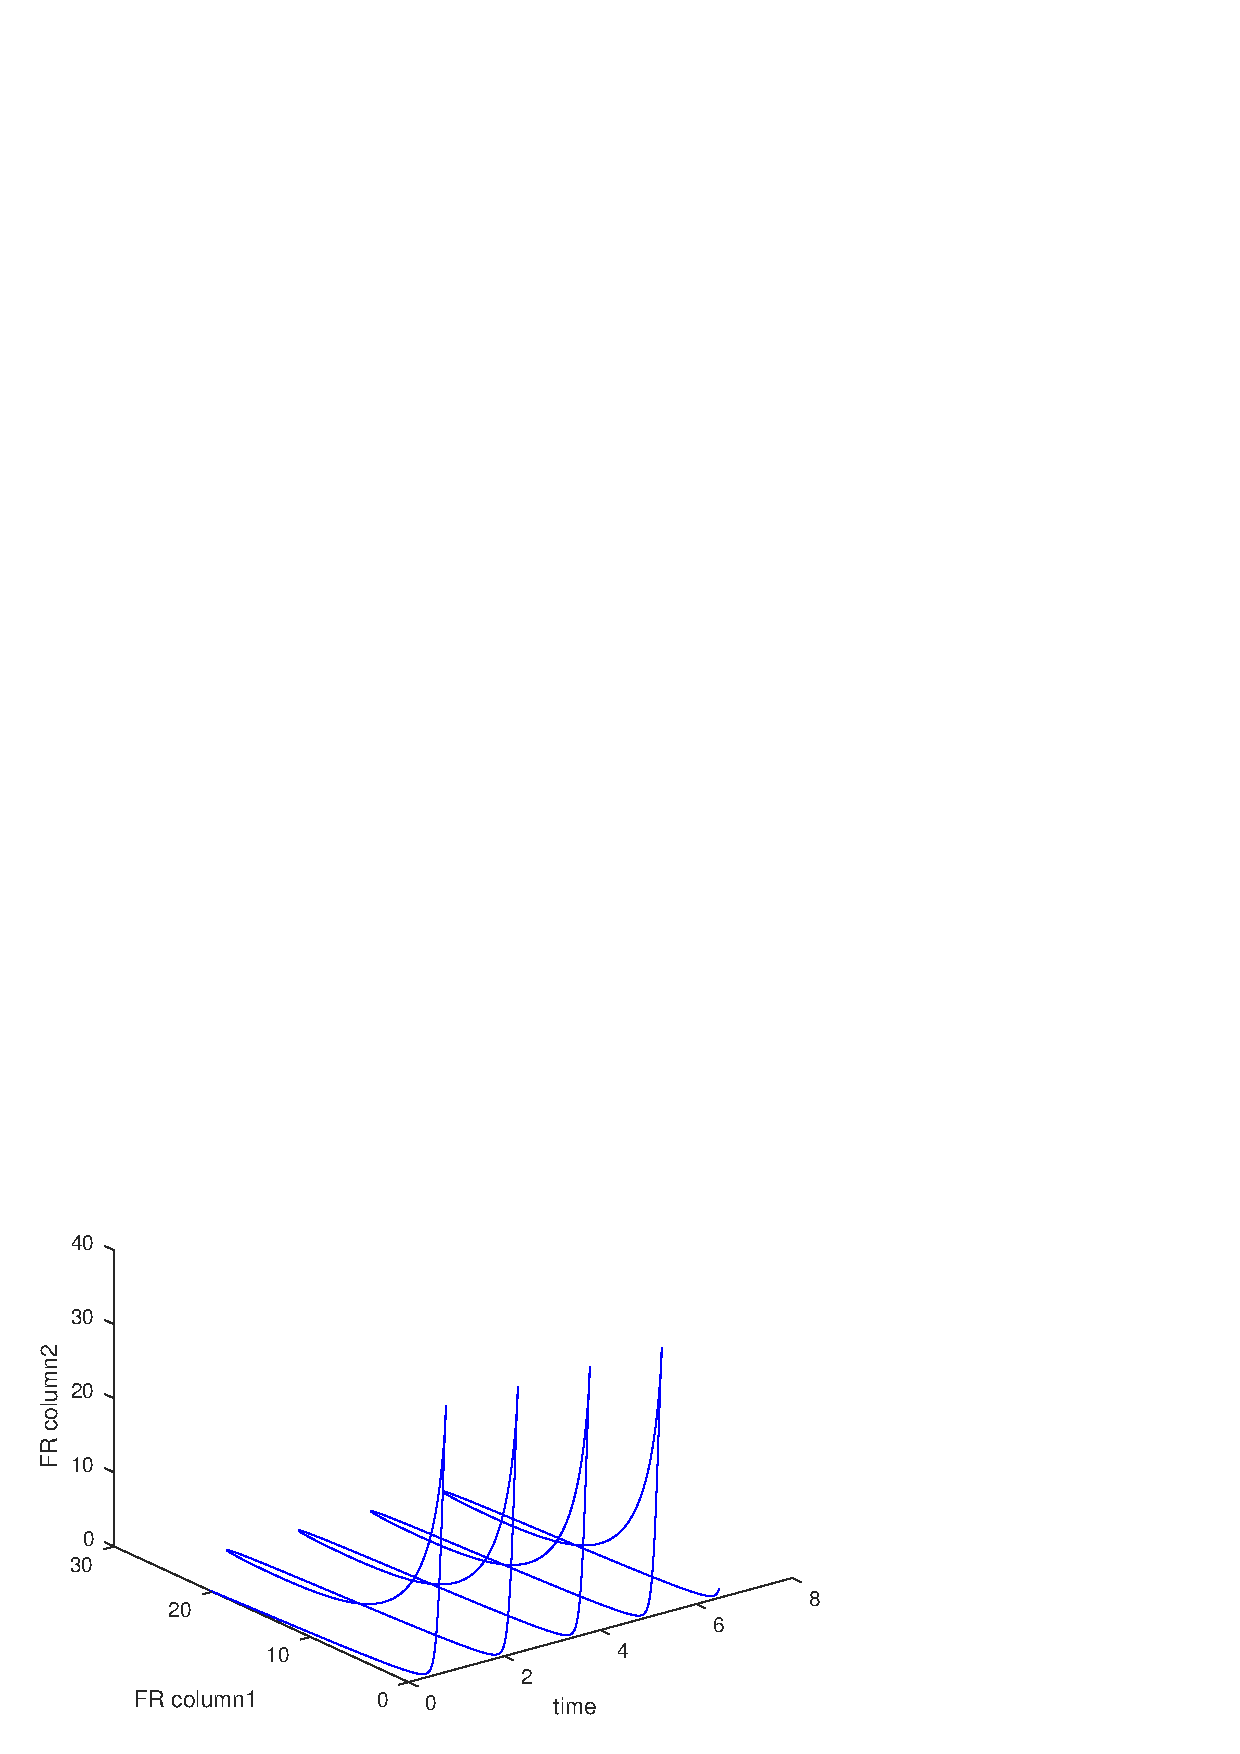
\includegraphics[width=\linewidth]{/home/tesylvia/Oral_Sept_2017/images/FinalOralPlots/SyntheticOralPaper/SimFiringRate-with-Time.pdf}
\caption{Simulated firing rate  data}\label{fig:SimFRwithTime}
\end{subfigure}

\begin{subfigure}[b]{.45\linewidth}
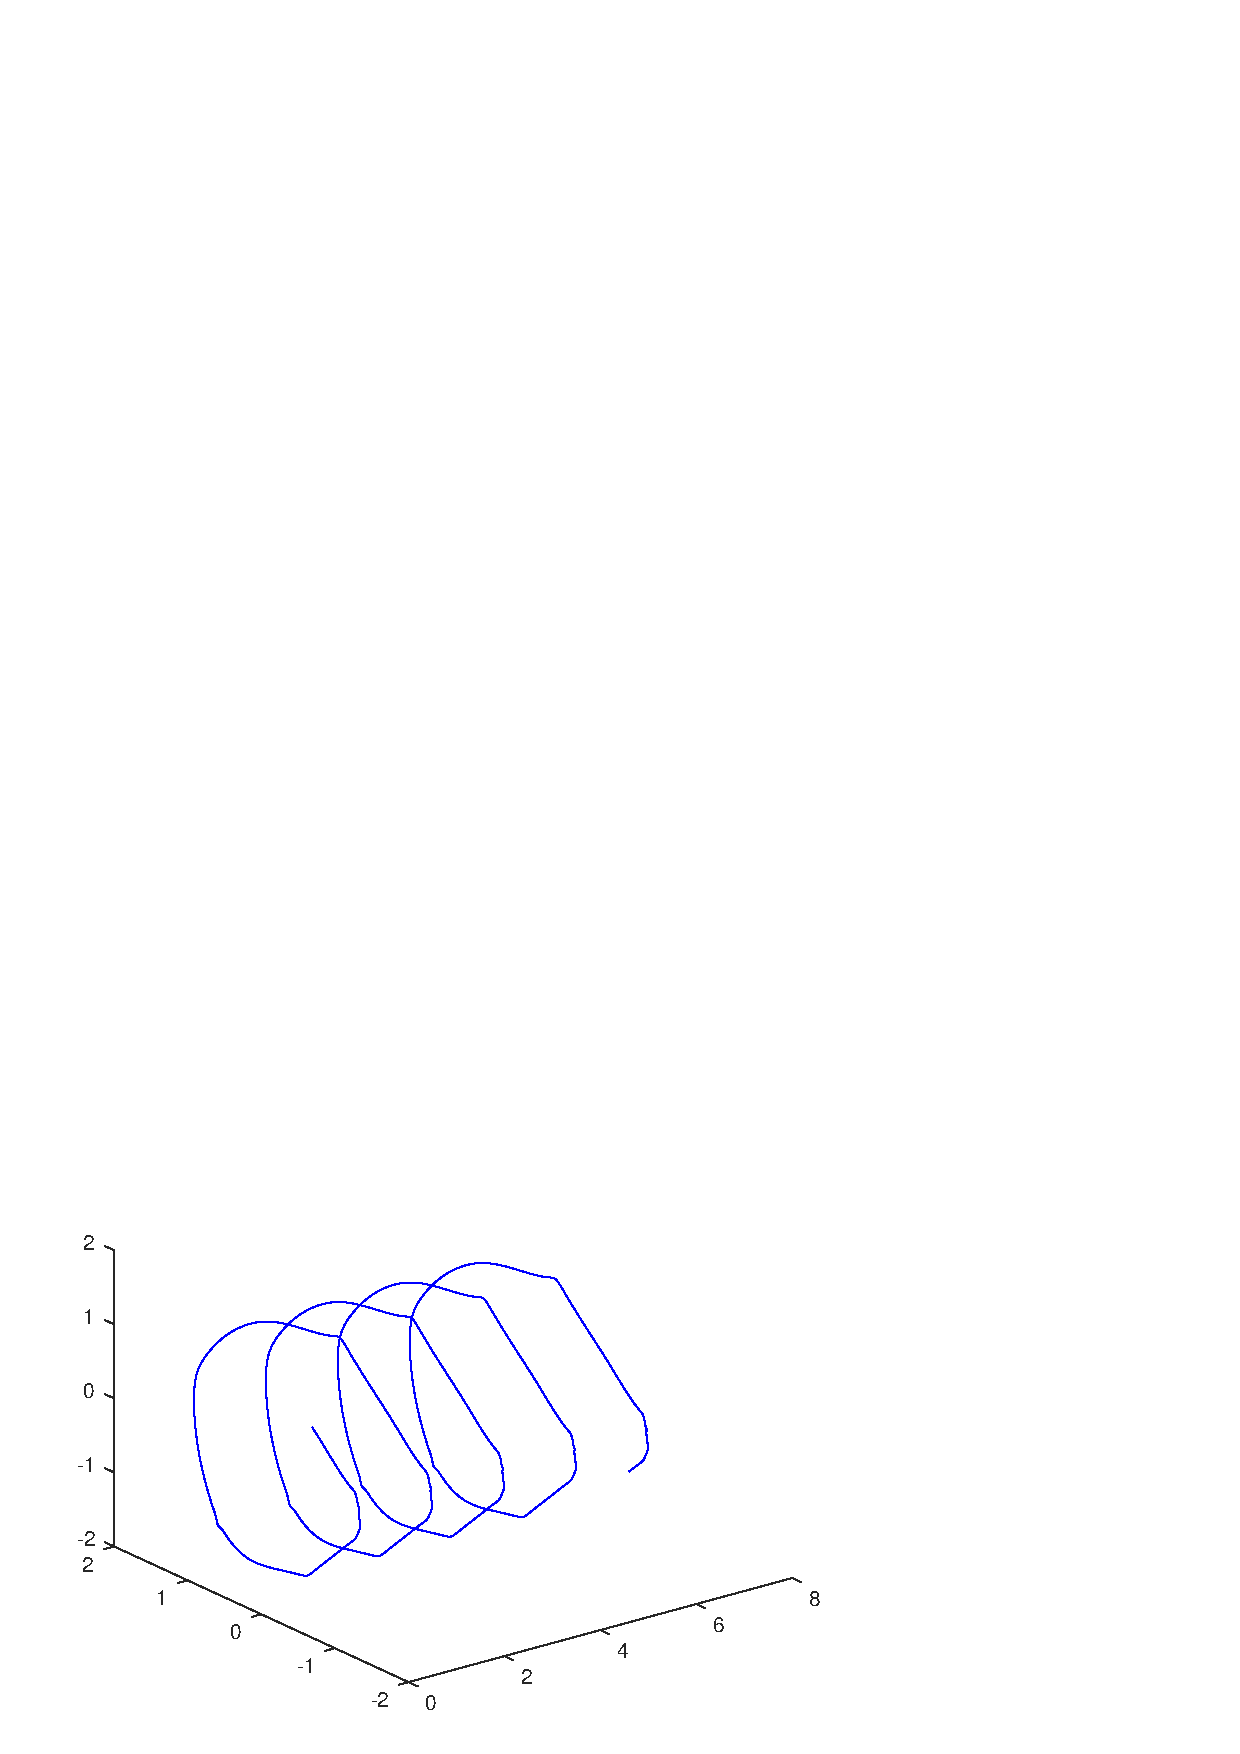
\includegraphics[width=\linewidth]{/home/tesylvia/Oral_Sept_2017/images/FinalOralPlots/SyntheticOralPaper/SimFRDML1-with-time.pdf}
\caption{Diffusion Maps on firing rate}\label{fig:SimFRDML1vsTime}
\end{subfigure}
\begin{subfigure}[b]{.45\linewidth}
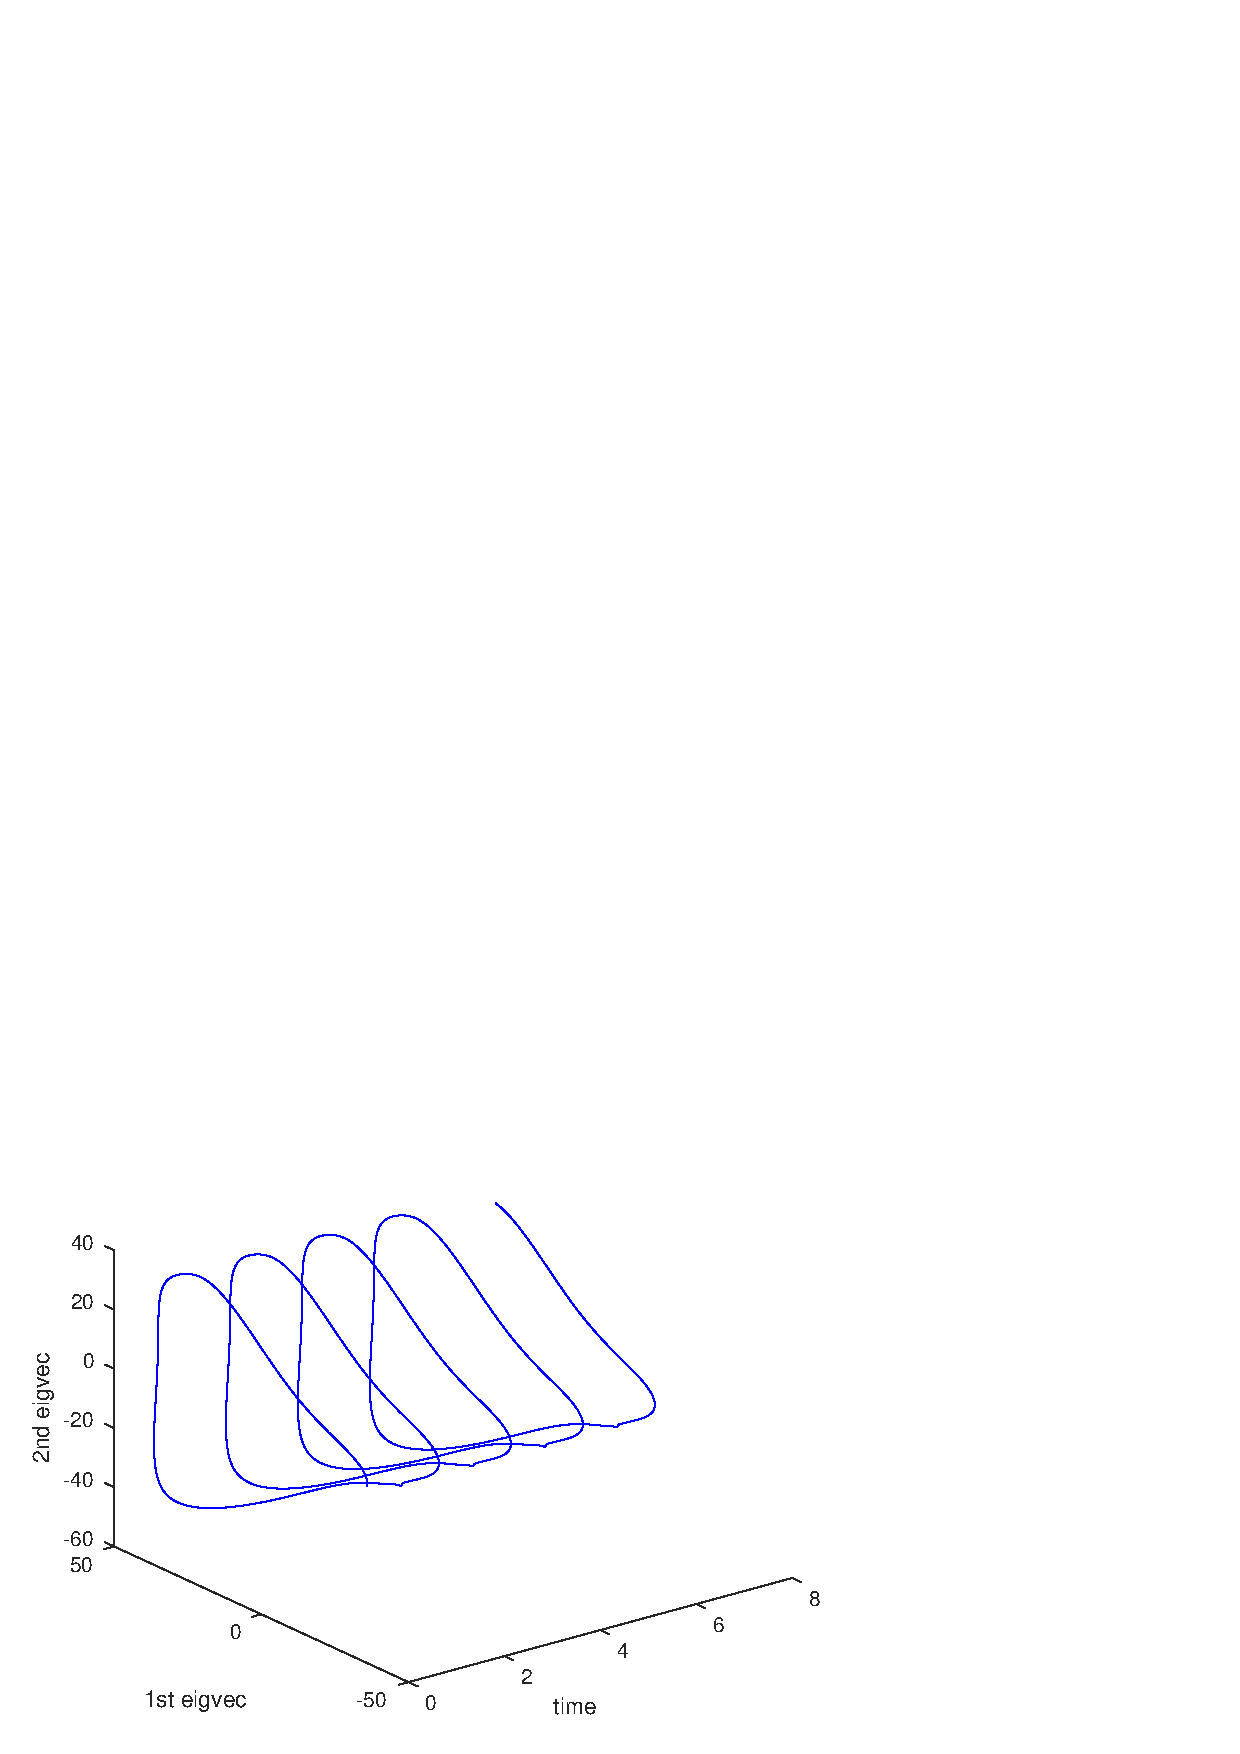
\includegraphics[width=\linewidth]{/home/tesylvia/Oral_Sept_2017/images/FinalOralPlots/SyntheticOralPaper/SimFRPCA-with-time.pdf}
\caption{PCA on  firing rate}\label{fig:SimFRPCAvsTime}
\end{subfigure}
\begin{subfigure}[b]{.45\linewidth}
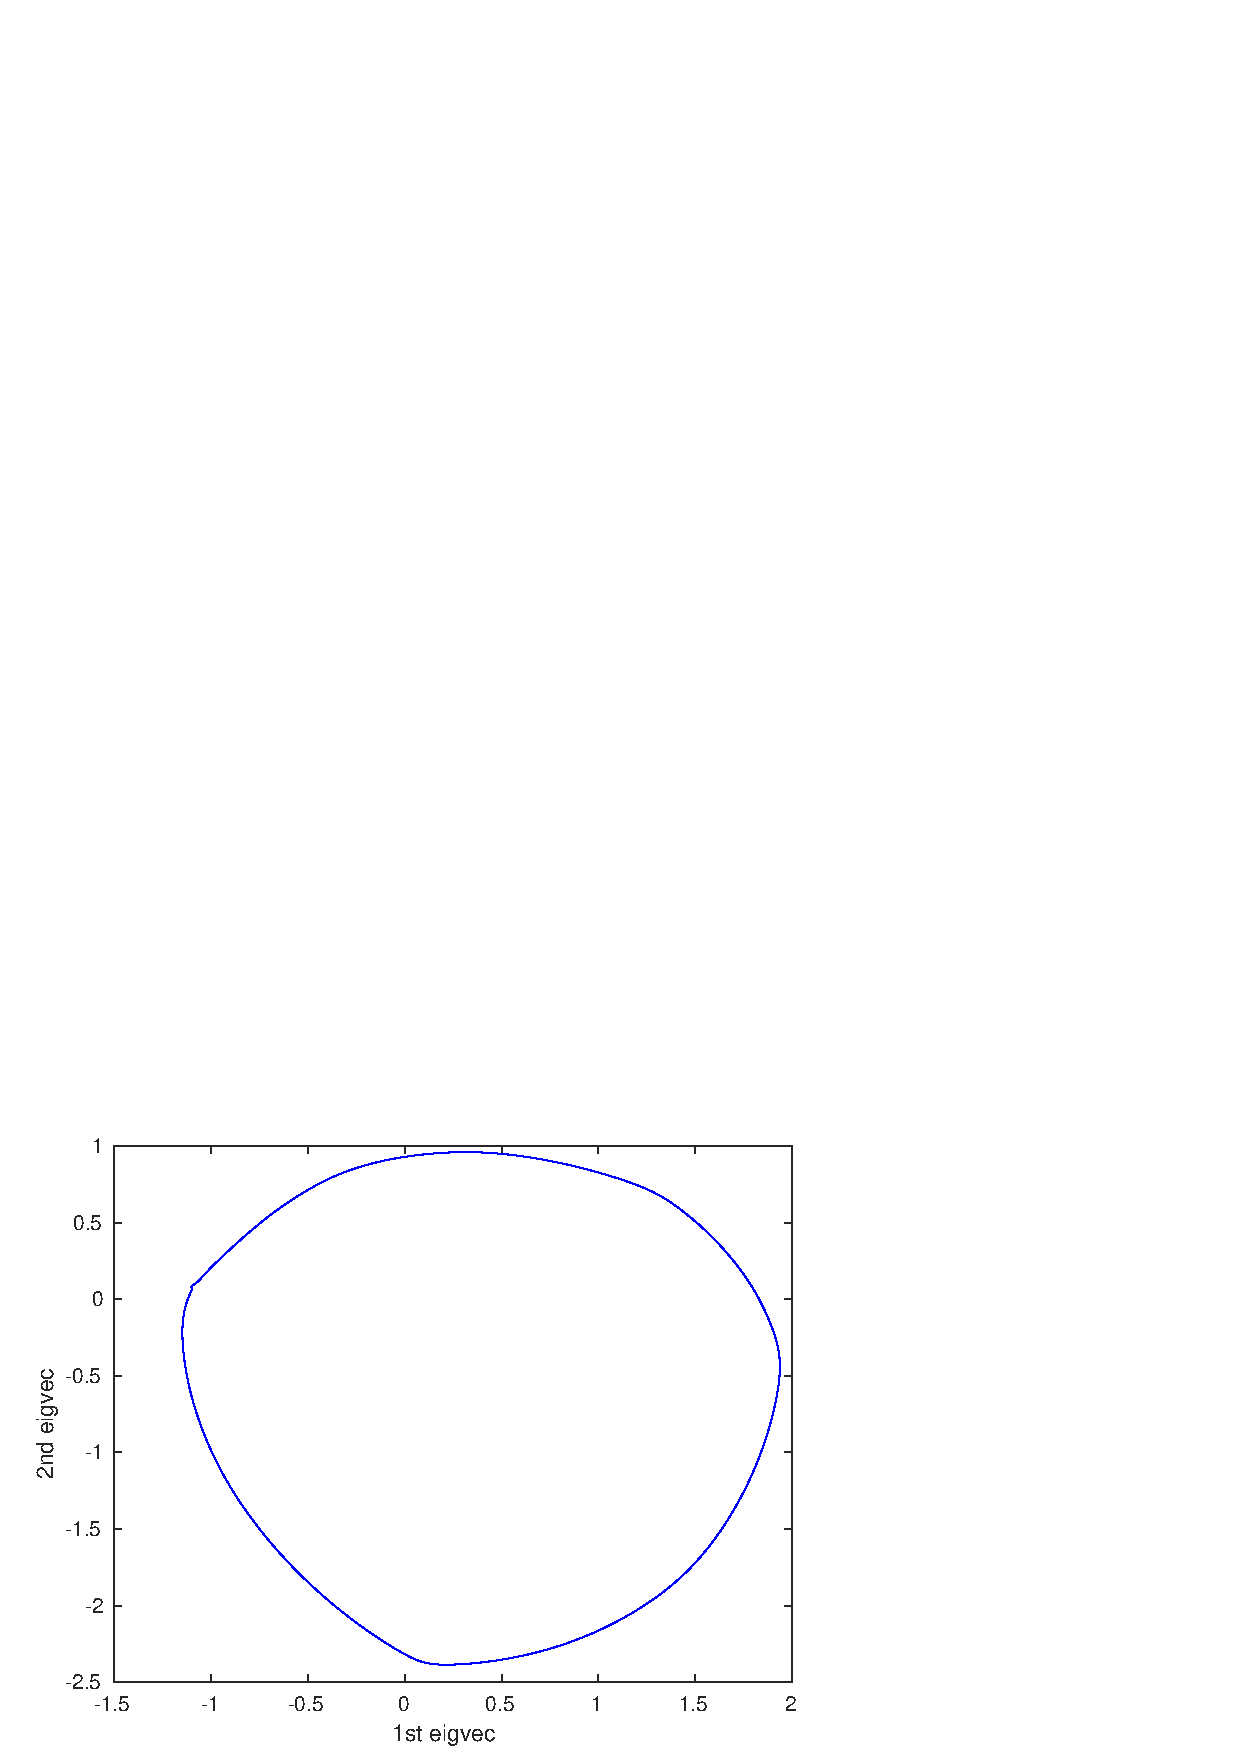
\includegraphics[width=\linewidth]{/home/tesylvia/Oral_Sept_2017/images/FinalOralPlots/SyntheticOralPaper/SimFRDML1.pdf}
\caption{Diffusion Maps on firing rate}\label{fig:SimFRDML1-2D}
\end{subfigure}
\begin{subfigure}[b]{.45\linewidth}
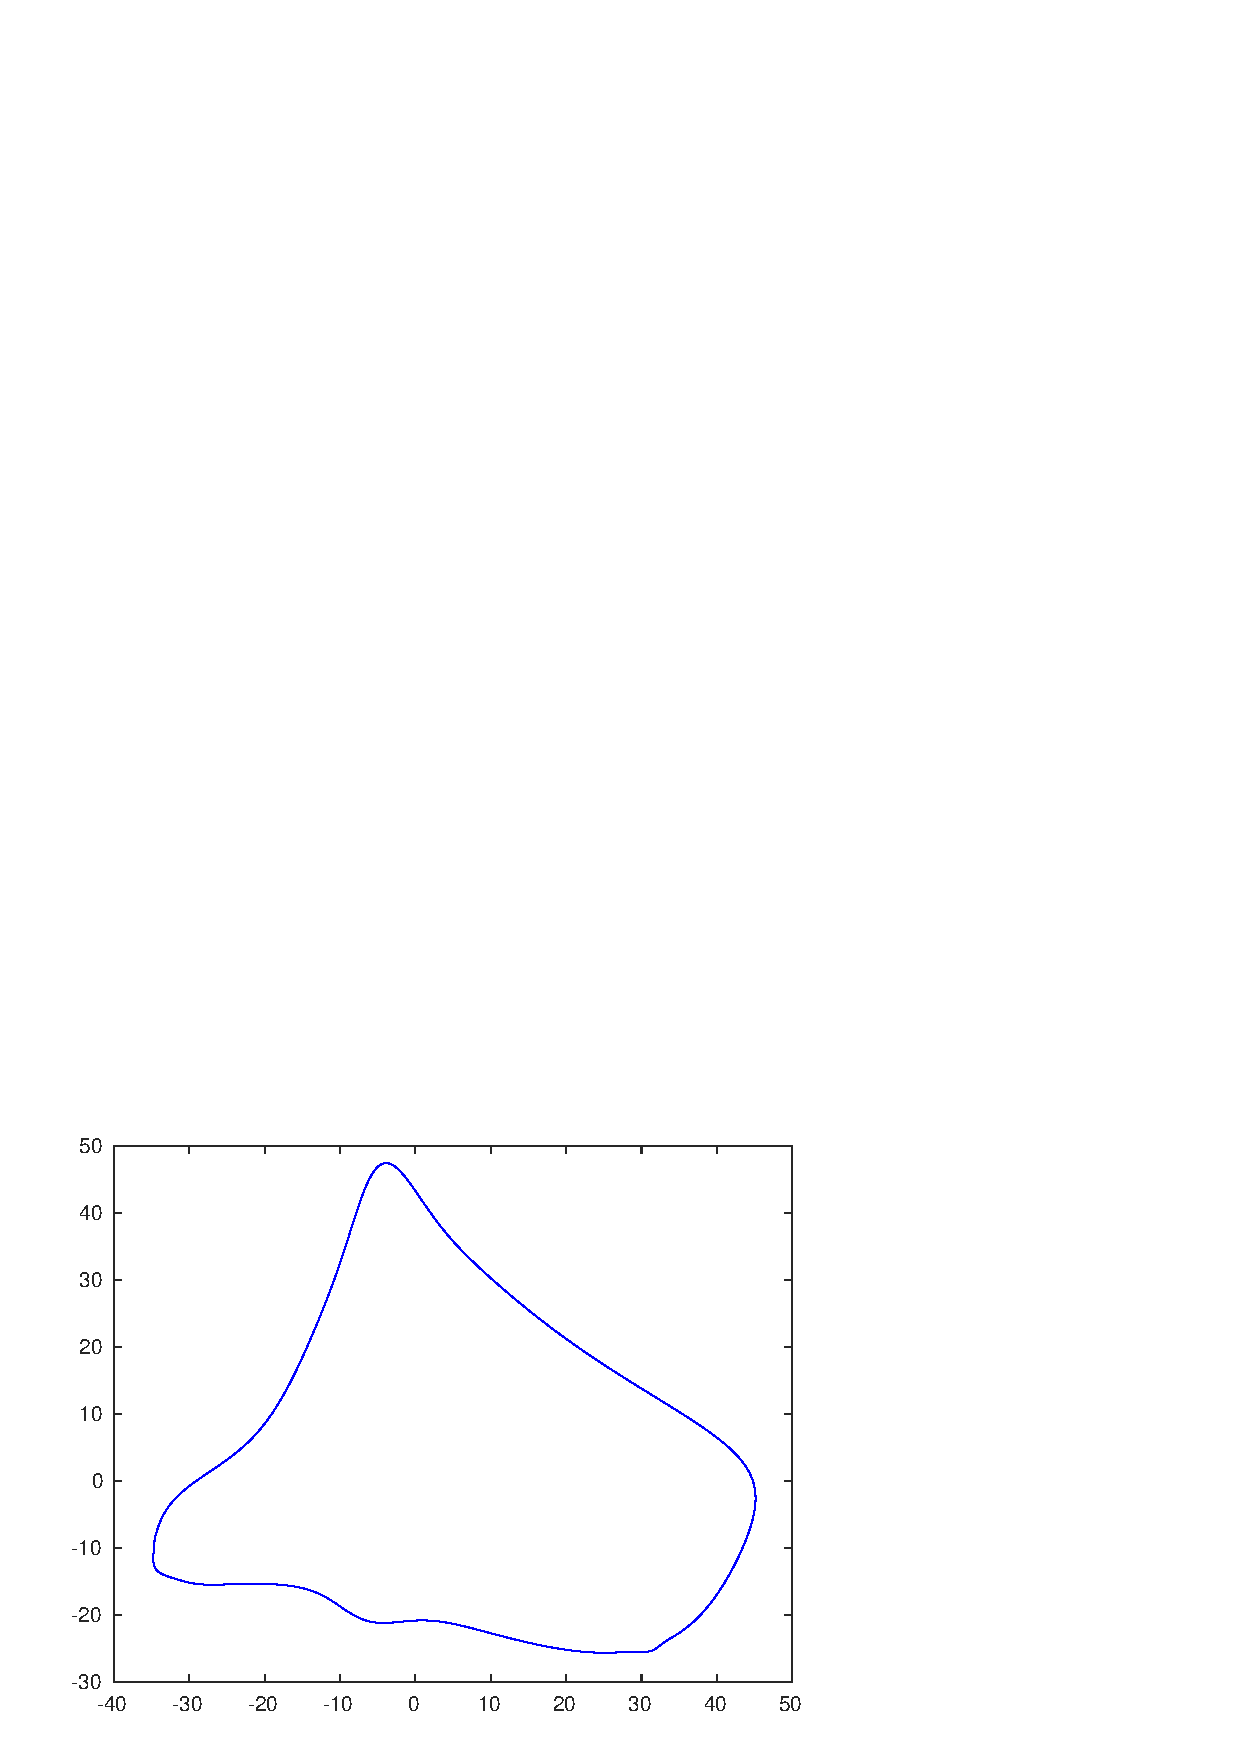
\includegraphics[width=\linewidth]{/home/tesylvia/Oral_Sept_2017/images/FinalOralPlots/SyntheticOralPaper/SimFRPCA.pdf}
\caption{PCA on firing rate}\label{fig:SimFRPCA-2D}
\end{subfigure}
\caption{Diffusion maps  with $l_{1}$ distance appears to capture the animal's circular motion better than PCA}
\label{fig:Output-on-SimFR}
\end{figure}

\newpage



\subsection{Simulation results on previous time data}
In this section, we show the results of diffusion maps with $l_{1}$ distance 
and PCA on simulated previous time data. 

\begin{figure}[h!]
\centering
\begin{subfigure}[b]{.45\linewidth}
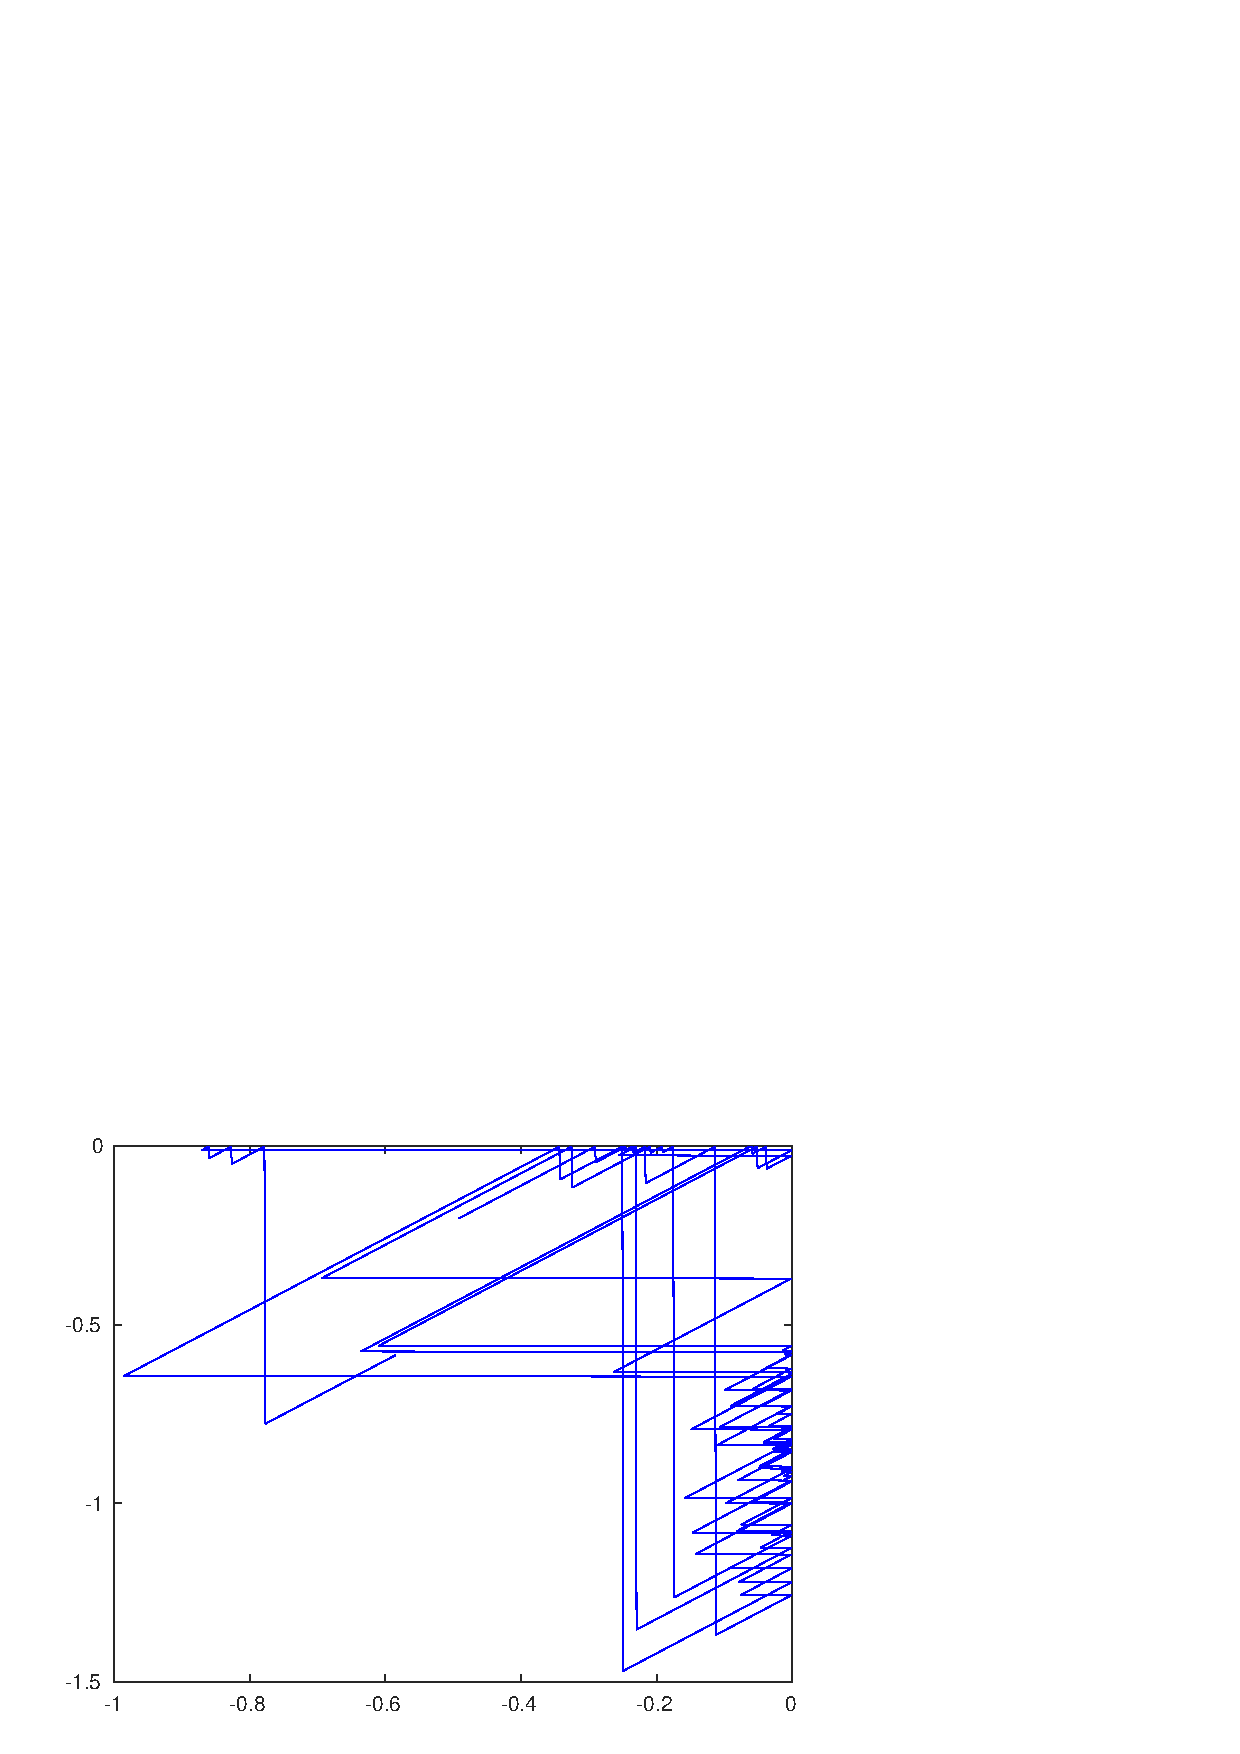
\includegraphics[width=\linewidth]{/home/tesylvia/Oral_Sept_2017/images/FinalOralPlots/SyntheticOralPaper/SimPrevtime.pdf}
\caption{Simulated previous time data}\label{fig:SimPrevtime}
\end{subfigure}
\begin{subfigure}[b]{.45\linewidth}
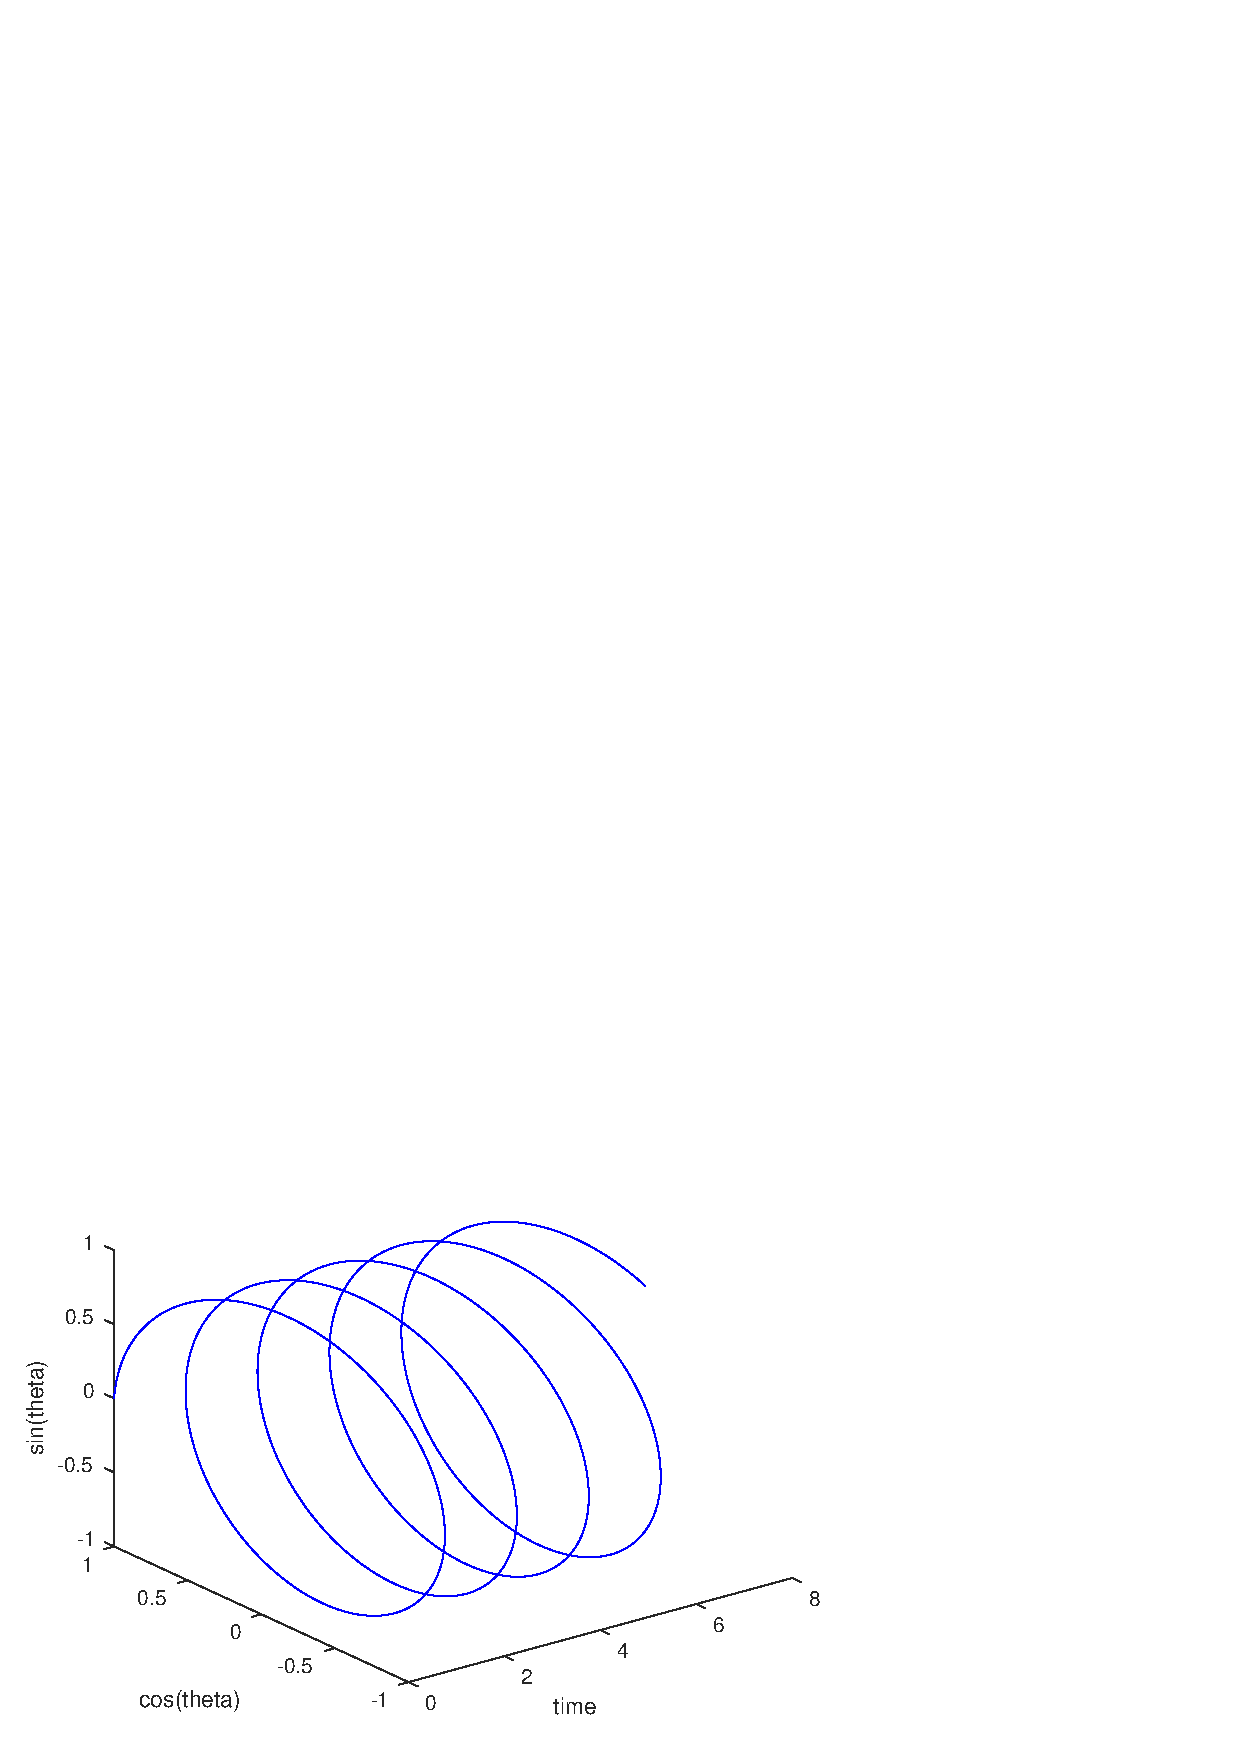
\includegraphics[width=\linewidth]{/home/tesylvia/Oral_Sept_2017/images/FinalOralPlots/SyntheticOralPaper/SimRatPosition.pdf}
\caption{Simulated animal position}\label{fig:SimPosition}
\end{subfigure}
\begin{subfigure}[b]{.45\linewidth}
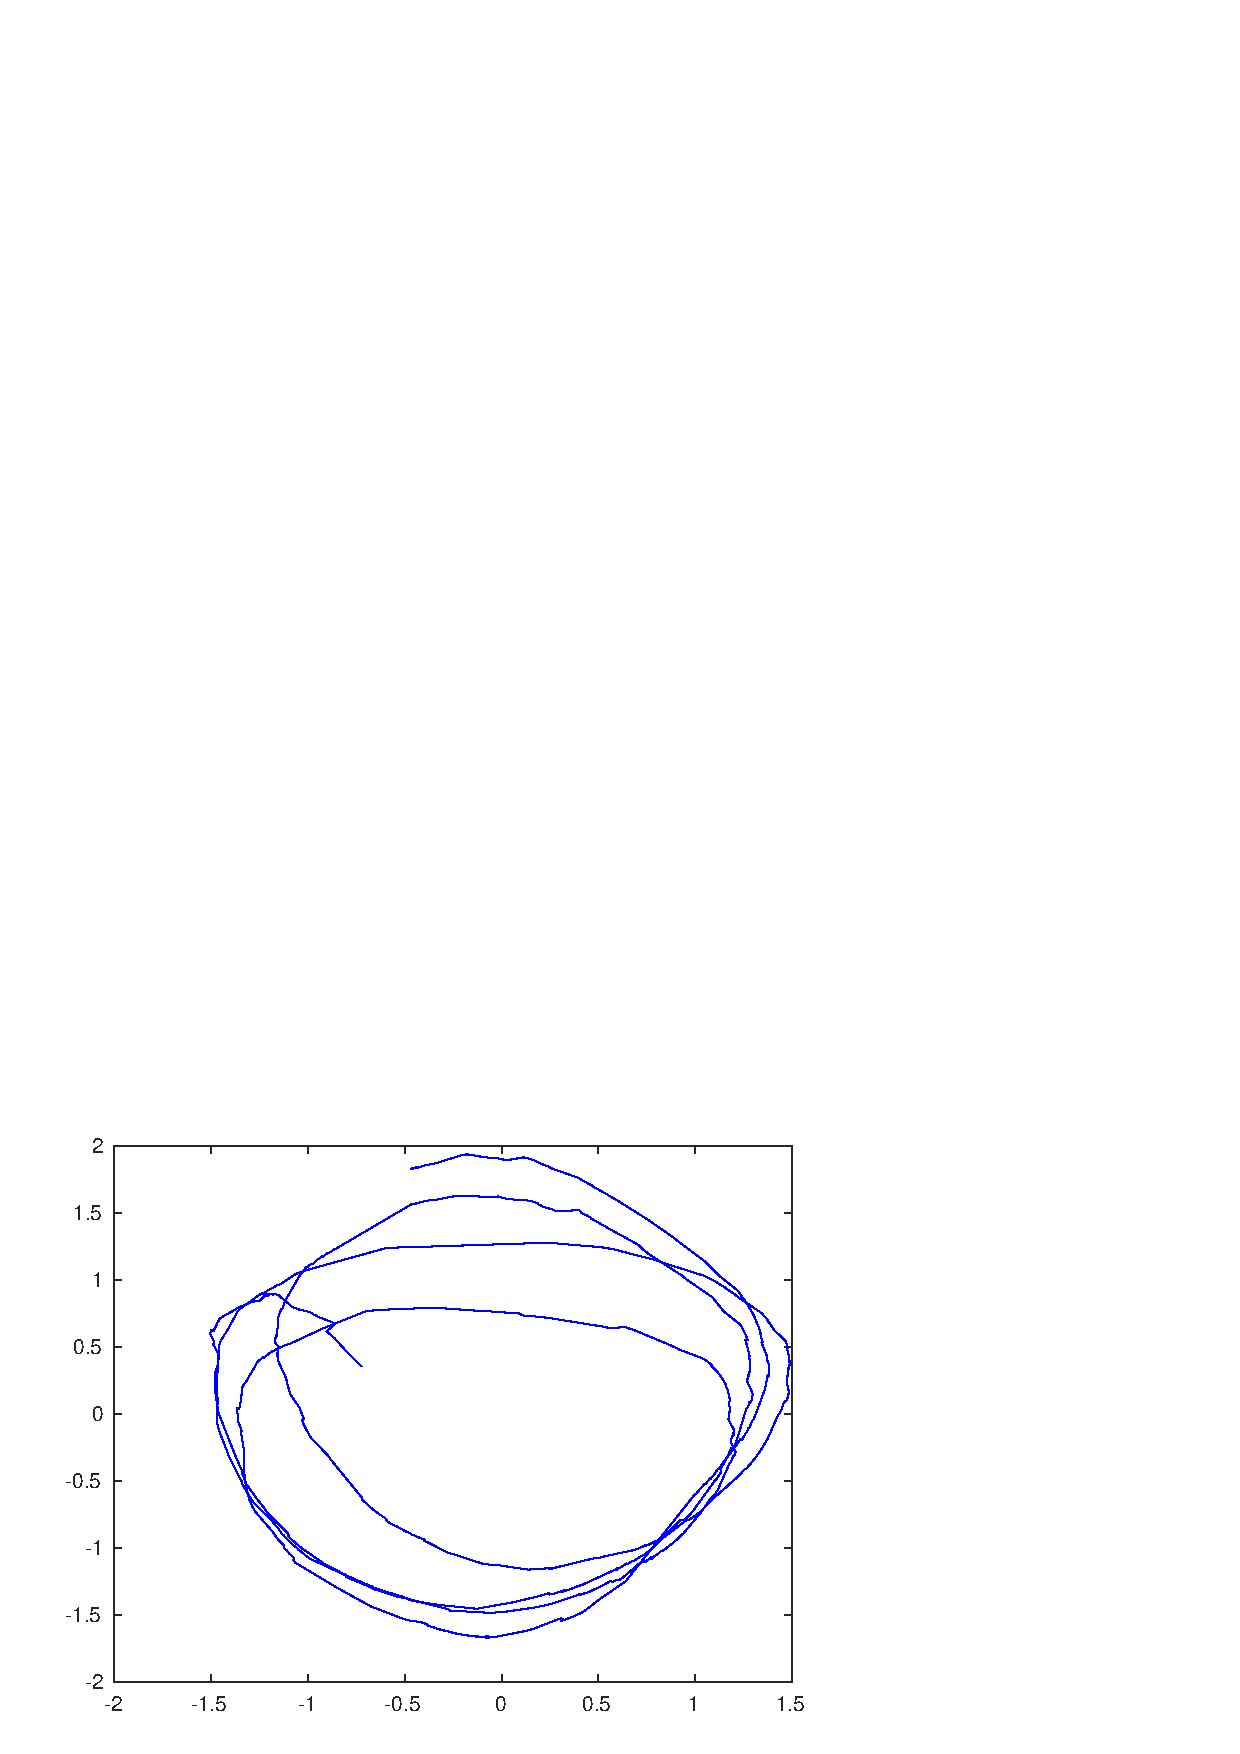
\includegraphics[width=\linewidth]{/home/tesylvia/Oral_Sept_2017/images/FinalOralPlots/SyntheticOralPaper/SimPrevtimeDML1.pdf}
\caption{Diffusion Maps on previous time}\label{fig:SimPrevtimeDML1-2D}
\end{subfigure}
\begin{subfigure}[b]{.45\linewidth}
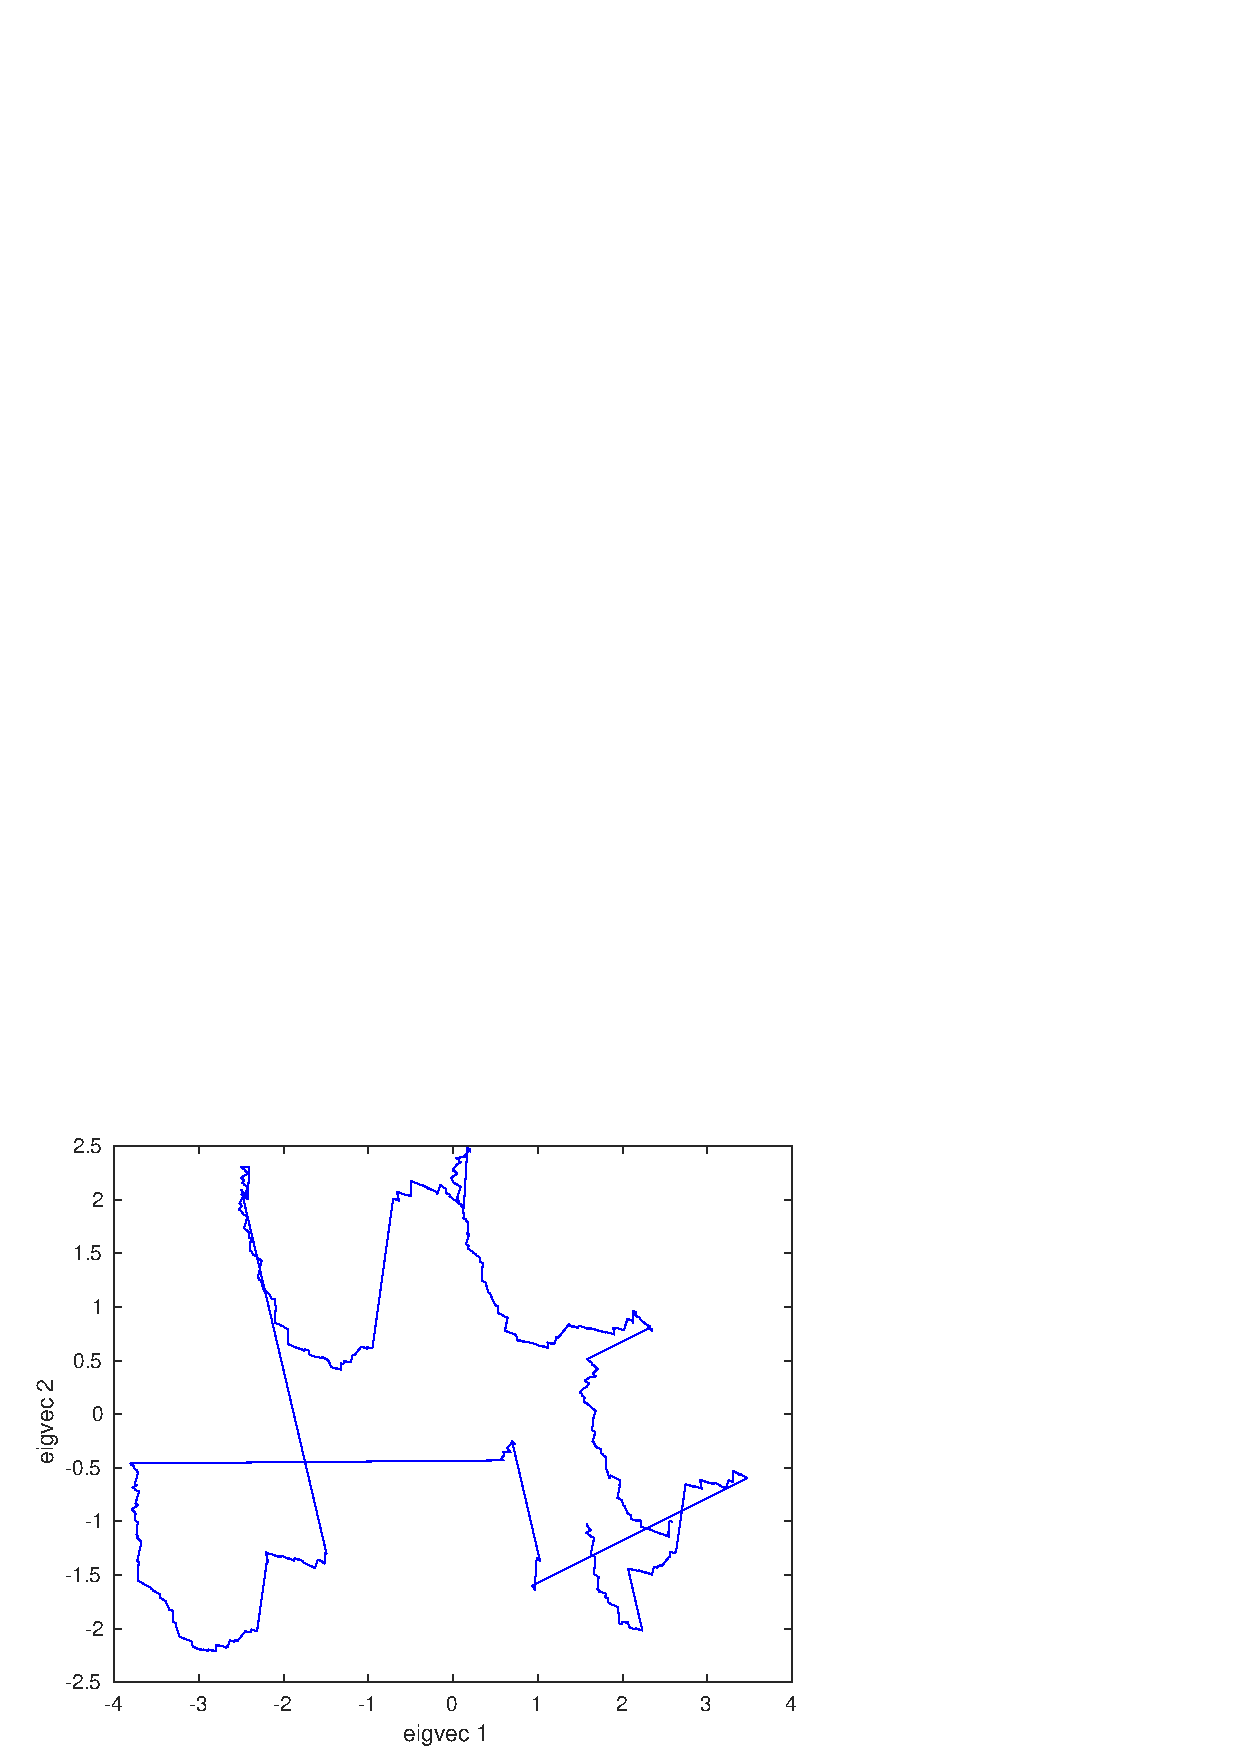
\includegraphics[width=\linewidth]{/home/tesylvia/Oral_Sept_2017/images/FinalOralPlots/SyntheticOralPaper/SimPrevtimePCA.pdf}
\caption{PCA on  previous time}\label{fig:SimPrevtimePCA-2D}
\end{subfigure}
\begin{subfigure}[b]{.45\linewidth}
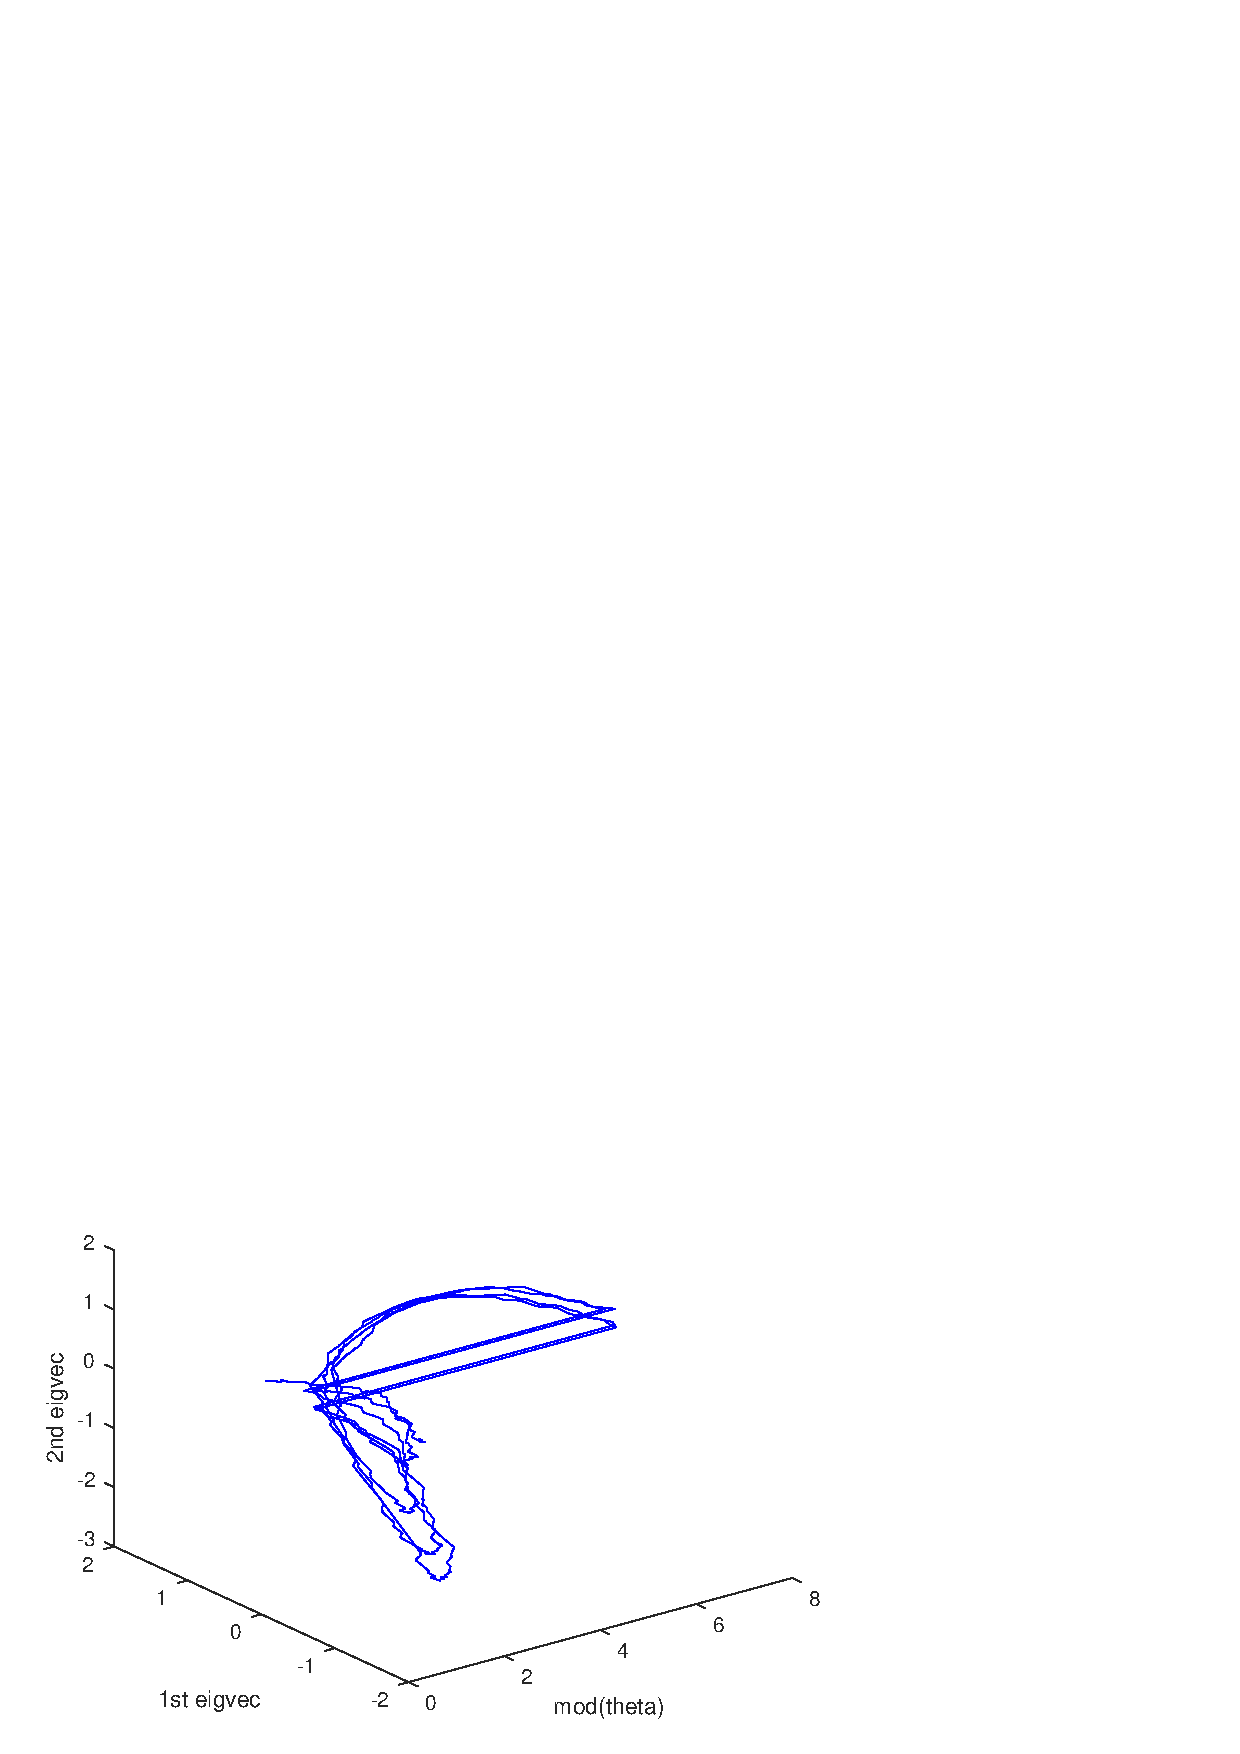
\includegraphics[width=\linewidth]{/home/tesylvia/Oral_Sept_2017/images/FinalOralPlots/SyntheticOralPaper/SimPrevtimeDML1-with-Position.pdf}
\caption{Diffusion Maps on previous time}\label{fig:SimPrevtimeDML1-3D}
\end{subfigure}
\begin{subfigure}[b]{.45\linewidth}
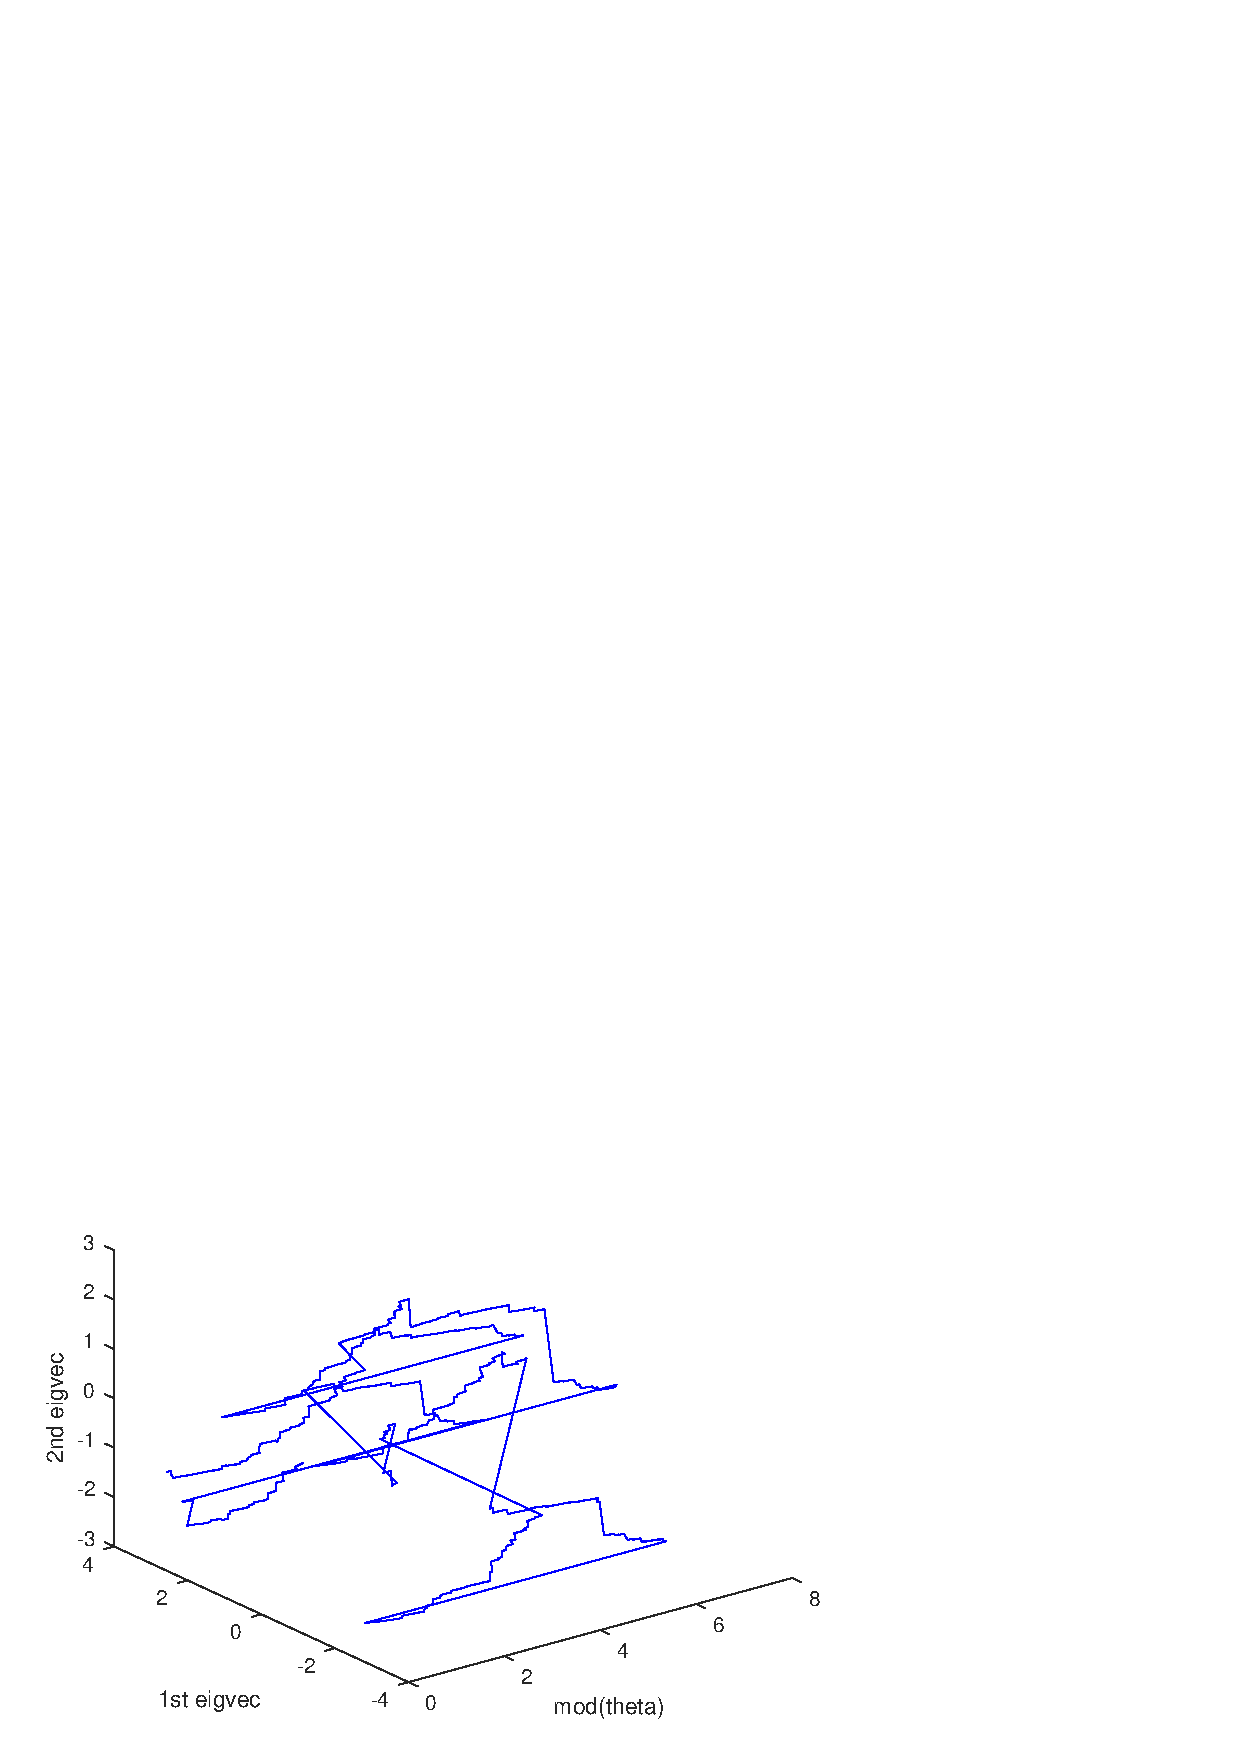
\includegraphics[width=\linewidth]{/home/tesylvia/Oral_Sept_2017/images/FinalOralPlots/SyntheticOralPaper/SimPrevtimePCA-with-Position.pdf}
\caption{PCA on previous time}\label{fig:SimPrevtimePCA-3D}
\end{subfigure}
\caption{Diffusion maps  with $l_{1}$ distance appears to accurately capture both the animal's circular motion and changes in spike timing compared to PCA.}
\label{fig:Output-on-SimPrevtime}
\end{figure}


































































%\begin{itemize}
%\item show the graphs/results package
%\item this is how we're interpreting the results
%\item why does this matter?
%\item what measure of goodness did you use?
%(Fisher Vs Shannon information)

%%==========suggested by Duane============================================
%\item Mention that there are other ways of checking measures of goodness
% e.g the one provided by diffusion maps, Bayesian decoding refer to the nature
% and review artcicle.


%\end{itemize}







